\documentclass{beamer}

\usetheme{metropolis}
\definecolor{mediumred}{RGB}{180, 10, 5}
\setbeamercolor{frametitle}{bg=mediumred, fg=white}

\usepackage{tkz-graph}
\usepackage{tikz}
\usetikzlibrary{arrows,matrix,decorations.pathreplacing,positioning,chains,fit,shapes,calc} %
\usetikzlibrary{calc,patterns,decorations.pathmorphing,decorations.markings}

\usepackage{siunitx}

\usepackage{../../latex/custom}

\title{Computing ellipsoidal controlled invariant sets for stochastic programming}
\author{Beno\^it Legat and Rapha\"el Jungers (UCLouvain)}

\makeatletter
\let\@@magyar@captionfix\relax
\makeatother

\begin{document}
\maketitle

\begin{frame}
  \frametitle{Contents}
  \tableofcontents
\end{frame}

\section{Relatively Complete Recourse}

\begin{frame}
  \frametitle{Motivation : Water Reservoir}
  \begin{itemize}
    \item $h_{\textnormal{min}} \le h \le h_{\textnormal{max}}$ : water height [\si{\meter}]
    \item $v_{\textnormal{min}} \le v \le v_{\textnormal{max}}$ : height increase rate [\si{\meter\per\second}]
    \item $u_{\textnormal{min}} \le u \le u_{\textnormal{max}}$ : $v$ increase rate [\si{\meter\per\second\squared}]
  \end{itemize}
  \begin{columns}
    \begin{column}{0.45\textwidth}
      \begin{align*}
        h_{k+1} & = h_k + v_k \Delta t\\
        v_{k+1} & = v_k + u_k \Delta t
      \end{align*}
    \end{column}
    \begin{column}{0.45\textwidth}
      \begin{center}
        \includegraphics[width=\textwidth]{reservoir.jpg}
      \end{center}
    \end{column}
  \end{columns}
\end{frame}

\begin{frame}
  \frametitle{Relatively complete recourse}
  \begin{block}{Risks of infeasibility}
    \begin{itemize}
      \item $h > h_{\textnormal{max}}$: Water \alert{spills}
      \item $h < h_{\textnormal{min}}$: Risk of electricity \alert{shortage}
    \end{itemize}

    Bounds on $u$ prevents \alert{last-minute} actions.

    No \alert{relatively complete recourse}!

    Shortage is catastrophic $\to$ need \alert{huge} penalty $\to$ huge Lipschitz constant $L$ $\to$ huge sample size
    \[
      N \geq \mathcal{O}(L^2 \log(L) \cdots)
    \]
    {
      \footnotesize
      Shapiro and Nemirovski, \emph{On complexity of stochastic programming problems},
      Continuous optimization, 2005
    }
  \end{block}
\end{frame}

\section{Controlled Invariant Sets}

\begin{frame}{Controlled invariant set}
  \begin{block}{Linear discrete control system}
    \[ x_{k+1} = A x_k + B u_k, \quad x_k \in X, u_k \in U \]
  \end{block}
  \begin{block}{Controlled invariant set}
    Set $S \subseteq X$ \emph{controlled invariant} iff
    \[ \forall x \in S, \exists u \in U \text{ such that } Ax + Bu \in S \]
  \end{block}
  \begin{block}{Safe Stochastic Programming}
    \begin{itemize}
      \item Compute controlled invariant set $S \subseteq{}$safe set.
      \item Add constraint: state${}\in S$.
    \end{itemize}
  \end{block}
\end{frame}

\begin{frame}
  \frametitle{Analytical controlled invariant set}
  \textbf{Symmetrization}: Assume $v_{\textnormal{min}} = -v_{\textnormal{max}}$ and $u_{\textnormal{min}} = -u_{\textnormal{max}}$ for simplicity.
  Assume $h_{\textnormal{min}} = -h_{\textnormal{max}}$ wlog.
  \begin{center}
    \includegraphics[trim=.2cm .2cm .2cm .2cm, clip, width=0.9\textwidth]{ReservoirAnalytical.pdf}
  \end{center}
\end{frame}


\begin{frame}{Representation of polyhedral sets}
  \begin{block}{\hrep}
    Representation of polyhedron $S$ as intersection of halfspaces:
    \[ S = \bigcap_{i=1}^m \{\, x \mid a_i^\Tr x \le \beta_i \,\}. \]
    \vspace{-2.5em}
    \begin{itemize}
      \item Computing $A^{-1} S$ is \alert{easy}: $a_i \to A^\Tr a_i$.
      \item Projection is \alert{hard}. Algorithms: Fourier-Motzkin, ...
    \end{itemize}
  \end{block}
  \begin{block}{\vrep}
    Representation of polyhedron $S$ as hull of points/rays:
    \[ S = \convexhull(x_1, \ldots, x_{m_x}) + \conichull(r_1, \ldots, r_{m_r}). \]
    \vspace{-3em}
    \begin{itemize}
      \item Computing $A S$ is \alert{easy}: $x \to A x$, $r \to A r$.
      \item Projection is \alert{easy}: project each point/ray.
    \end{itemize}
  \end{block}
  \vspace{-1em}
  Representation conversion is \alert{hard}. Algorithms: double description,
  quick hull, ...
\end{frame}

\begin{frame}{Unconstrained input without loss of generality}
  \begin{block}{\alert{Constrained} input}
    \[ x_{k+1} = A x_k + B u_k, \quad x_k \in X, \alert{u_k \in U} \]
  \end{block}
  \textbf{\alert{Lift} to \alert{un}constrained input}: $x' = (x, u)$
  \begin{align*}
    x_{k+1} & =
    \begin{pmatrix}
      A & B
    \end{pmatrix}
    x'_k\\
    u_{k+1} & =
    u'_k
  \end{align*}
  where $x'_k \in X' = X \times U$.
\end{frame}


\begin{frame}{Computation of invariant set}
  \vspace{-.5em}
  Linear discrete system : \( x_{k+1} = A x_k \), $x_k \in X$.
  \vspace{-.8em}
  \begin{block}{Pre-image}
    \[ A^{-1}S \triangleq \{\, x \mid Ax \in S \,\} \]
  \end{block}
  \vspace{-.8em}
  \begin{block}{Invariant set}
    Set $S \subseteq X$ \emph{invariant} iff
    \begin{align*}
      \forall x \in S, Ax & \in S &\Leftrightarrow&& AS & \subseteq S &\Leftrightarrow&& S & \subseteq A^{-1}S
    \end{align*}
  \end{block}
  \only<2>{
  \vspace{-.8em}
    \begin{block}{\alert{Polyhedral} computation}
      \begin{align*}
        P_0 & = X\\
        P_{k+1} & = P_k \cap A^{-1} P_k
      \end{align*}
      \vspace{-3em}
      \begin{center}
        \begin{tabular}{ll}
          $A^{-1}$ & easy with \alerthrep\\
          $\cap$   & easy with \alerthrep
        \end{tabular}
      \end{center}
    \end{block}
  }
  \only<3>{
    \begin{block}{\alert{Ellipsoidal} computation}
      \[ C = \{\, x \mid x^\Tr Q x \le 1 \,\} \quad \Rightarrow \quad A^{-1}C = \{\, x \mid x^\Tr A^\Tr Q A x \le 1 \,\} \]
      S-procedure:
      \[ Q - A^\Tr Q A \text{ is PSD}. \]
    \end{block}
  }
\end{frame}

\begin{frame}{Polyhedral computation of controlled invariant set}
  \vspace{-1em}
  \begin{align*}
    P_0 & = X\\
    P_{k+1}
    & = P_k \cap \proj_x \{\, (x, u) \mid Ax + Bu \in P_k \,\}\\
    & = P_k \cap \proj_x [A, B]^{-1} P_k
  \end{align*}
  \vspace{-1em}
  \begin{block}{Not scalable...}
    \begin{center}
      \begin{tabular}{ll}
        $[A, B]^{-1}$ & easy with \alerthrep\\
        $\proj_x$     & easy with \alertvrep\\
        $\cap$        & easy with \alerthrep
      \end{tabular}
    \end{center}
  \end{block}
\end{frame}

\begin{frame}{Unconstrained control to algebraic system}
  \begin{block}{Linear Discrete \alert{Control} System (DT\alert{C}S)}
    \[ x_{k+1} = A x_k + B u_k, \quad x_k \in X \]
  \end{block}
  \begin{block}{Linear Discrete \alert{Algebraic} System (DT\alert{A}S)}
    \[ Ex_{k+1} = A x_k, \quad x_k \in X \]
    Invariant Set $S \subseteq X$ if
    \[ \forall x \in S, \alert{\exists} y \in S : Ey = Ax \]
  \end{block}
  \begin{block}{Reduction}
    The set $S$ is controlled invariant for the DT\alert{C}S iff
    it is invariant for the DT\alert{A}S
    \[ \Pi x_{k+1} = \Pi A x_k, \quad x_k \in X \]
    where $\Pi$ is a projection on $\Image(B)^\perp$.
  \end{block}
\end{frame}


\include{ellipsoid_algebraic_invariant}


\begin{frame}
  \frametitle{Result for reservoir}
  \begin{center}
    \includegraphics[trim=.2cm .2cm .2cm .2cm, clip, width=\textwidth]{ReservoirEllipsoidal.pdf}
  \end{center}
  \vspace{-1em}
  \uncover<2>{\includegraphics[width=0.1\textwidth]{Brazil.png}}
\end{frame}

\section{Hybrid Systems}

\begin{frame}
  \frametitle{Multistage Stochastic Program to Hybrid System}
  \begin{block}{Precomputing controlled invariant set}
    \alert{Feasibility only}, no objective function.

    Stochastic Program can be transformed to \alert{Hybrid} System.
  \end{block}

  \begin{center}
    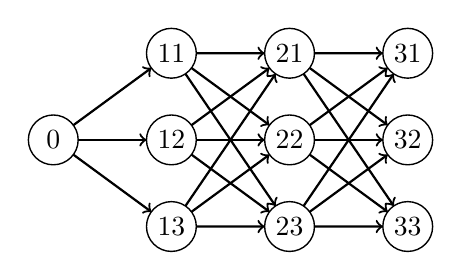
\begin{tikzpicture}[xscale=1.5, yscale=1.1]
      \Vertex{0}
      \NOEA(0){11};
      \EA  (0){12};
      \SOEA(0){13};
      \NOEA(12){21};
      \EA  (12){22};
      \SOEA(12){23};
      \NOEA(22){31};
      \EA  (22){32};
      \SOEA(22){33};
      \tikzset{EdgeStyle/.style={->}}
      \Edge(0)(11)
      \Edge(0)(12)
      \Edge(0)(13)
      \Edge(11)(21)
      \Edge(11)(22)
      \Edge(11)(23)
      \Edge(12)(21)
      \Edge(12)(22)
      \Edge(12)(23)
      \Edge(13)(21)
      \Edge(13)(22)
      \Edge(13)(23)
      \Edge(21)(31)
      \Edge(21)(32)
      \Edge(21)(33)
      \Edge(22)(31)
      \Edge(22)(32)
      \Edge(22)(33)
      \Edge(23)(31)
      \Edge(23)(32)
      \Edge(23)(33)
    \end{tikzpicture}
    ~\hfill~
    \begin{tikzpicture}[xscale=1.5, yscale=1.1]
      \Vertex{0}
      \Edge(0)(11)
      \NOEA(0){1}
      \EA  (0){2}
      \SOEA(0){3}
      \tikzset{EdgeStyle/.style={->}}
      \Edge(0)(1)
      \Edge(0)(2)
      \Edge(0)(3)
      \Loop[dist=1.5em,dir=NO](1)
      \Loop[dist=1.5em,dir=EA](2)
      \Loop[dist=1.5em,dir=SO](3)
      \tikzset{EdgeStyle/.style={->, bend left=15}}
      \Edge(1)(2)
      \Edge(2)(1)
      \Edge(2)(3)
      \Edge(3)(2)
      \tikzset{EdgeStyle/.style={->, bend left}}
      \Edge(1)(3)
      \Edge(3)(1)
    \end{tikzpicture}
  \end{center}
\end{frame}

\begin{frame}{Controlled invariant set for Hybrid Systems}
  Four speed limits with a delay $T$ to satisfy limit\\$\to$ \alert{Hybrid} System

  \begin{center}
    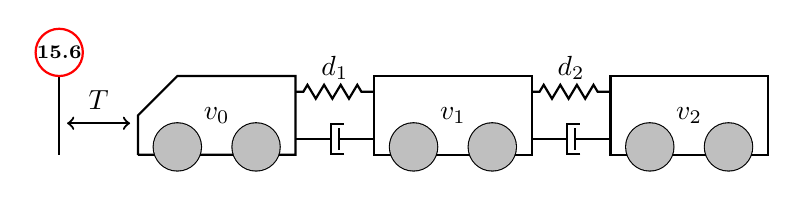
\begin{tikzpicture}
      \tikzstyle{spring}=[thick,decorate,decoration={zigzag,pre length=0.1cm,post length=0.1cm,segment length=6}]
\tikzstyle{damper}=[thick,decoration={markings,
  mark connection node=dmp,
  mark=at position 0.5 with
  {
    \node (dmp) [thick,inner sep=0pt,transform shape,rotate=-90,minimum width=10pt,minimum height=2pt,draw=none] {};
    \draw [thick] ($(dmp.north east)+(2pt,0)$) -- (dmp.south east) -- (dmp.south west) -- ($(dmp.north west)+(2pt,0)$);
    \draw [thick] ($(dmp.north)+(0,-4pt)$) -- ($(dmp.north)+(0,4pt)$);
  }
}, decorate]
\draw[thick] (0, 0) -- (2, 0) -- (2, 1) -- (0.5, 1) -- (0, 0.5) -- (0, 0);
\draw [spring] (2, 0.8) -- (3, 0.8);
\draw [damper] (2, 0.2) -- (3, 0.2);
\draw[thick] (3, 0) rectangle (5, 1);
\draw [spring] (5, 0.8) -- (6, 0.8);
\draw [damper] (5, 0.2) -- (6, 0.2);
\draw[thick] (6, 0) rectangle (8, 1);
\draw[thick] (0.5, 0.1) circle (0.3);
\fill[color=lightgray] (0.5, 0.1) circle (0.3);
\draw[thick] (1.5, 0.1) circle (0.3);
\fill[color=lightgray] (1.5, 0.1) circle (0.3);
\draw[thick] (3.5, 0.1) circle (0.3);
\fill[color=lightgray] (3.5, 0.1) circle (0.3);
\draw[thick] (4.5, 0.1) circle (0.3);
\fill[color=lightgray] (4.5, 0.1) circle (0.3);
\draw[thick] (6.5, 0.1) circle (0.3);
\fill[color=lightgray] (6.5, 0.1) circle (0.3);
\draw[thick] (7.5, 0.1) circle (0.3);
\fill[color=lightgray] (7.5, 0.1) circle (0.3);
\node at (1, 0.5) {$v_0$};
\node at (4, 0.5) {$v_1$};
\node at (7, 0.5) {$v_2$};
\node at (2.5, 1.1) {$d_1$};
\node at (5.5, 1.1) {$d_2$};

      \draw[thick] (-1, 0) to (-1, 1);
      \draw[thick,color=red] (-1, 1.3) circle (0.3);
      \node at (-1, 1.3) {\scriptsize \bf 15.6};
      \draw[thick, <->] (-0.9, 0.4) to (-0.1, 0.4);
      \node at (-0.5, 0.7) {$T$};
    \end{tikzpicture}
  \end{center}

  Generalization to Hybrid Systems:

  {\scriptsize
  L., B.; Tabuada, P. \& Jungers, R. M.\\
  Computing controlled invariant sets for hybrid systems with applications to model-predictive control.\\
  \emph{Proceedings of the IFAC Conference on Analysis and Design of Hybrid Systems}, \textbf{2018}}
\end{frame}

\begin{frame}{Results for Hybrid Systems}
  \begin{columns}
    \begin{column}{0.55\textwidth}
      \begin{center}
        \includegraphics[width=\textwidth]{CruiseControlSets.pdf}
        \includegraphics[width=\textwidth]{CruiseControlBenchmark.png}
      \end{center}
    \end{column}
    \begin{column}{0.55\textwidth}
      \begin{center}
        \includegraphics[width=\textwidth]{CruiseControlSpeed.pdf}
        \includegraphics[width=\textwidth]{CruiseControlAcceleration.pdf}
      \end{center}
    \end{column}
  \end{columns}
\end{frame}

\section{Conclusion}

\begin{frame}
  \frametitle{Conclusion and future work}
  \begin{block}{Conclusion}
    \begin{itemize}
      \item Solving stochastic problems without relatively complete recourse is \alert{difficult}.
      \item Need to compute maximal \alert{controlled invariant} sets of an \alert{hybrid} system.
      \item \alert{Ellipsoidal} controlled invariant sets can be computed using \alert{SDP}.
    \end{itemize}
  \end{block}
  \begin{block}{Future work}
    \begin{itemize}
      \item \alert{Semialgebraic} invariant sets using \alert{Sum-of-Squares}.
      \item Improve \alert{BMI} optimization for \alert{non-symmetric} case.
      \item \alert{Piecewise} quadratic invariant set.
    \end{itemize}
  \end{block}
\end{frame}

\end{document}
